\section{Kreuzvorhersage}
\label{sec:exp_cross_pred}
Momentan ist es durch in vitro Experimente bereits möglich die Ausbreitung der elektrischen Erregung auf der Oberfläche des Herzmuskels experimentell aufzuzeichnen. In Folge dessen stellt sich die Frage, ob anhand beispielsweise der Messung der Membramspannung weitere Variablen des Systems, wie die Kalium-Konzentration oder ähnliches, ermittelt werden können. Diese Fragestellung wird in dem ersten Szenario betrachtet. Es wird die Vorhersage von der Spannungsvariable auf die zweite Variable des jeweiligen Modells sowohl für das \textit{Barkley}- als auch für das \textit{Mitchell-Schaeffer}-Modell durchgeführt. Dabei wird zuerst die \textit{Nächste-Nachbar}-Methode, anschließend die \textit{radialen Basisfunktionen} und schlussendlich die \textit{ESN}s verwendet. Die daraus resultierenden Ergebnisse werden einzeln präsentiert und anschließend einem abschließenden Vergleich unterzogen.
 
\subsection{Nächste Nachbar Vorhersage}
Die Ergebnisse für die optimalen Hyperparameter des Ansatzes $\delta \in \{3,4,5\}, k \in \{2, 3, 4, 5\}$ sind in Tabelle \ref{tab:exp_cross_nn_results} zu finden. Dabei steht $k$ für die Anzahl der nächsten Nachbarn, welche für die Vorhersage genutzt werden und $\delta$ für die zusätzliche Dimensionalität durch die Verzögerungskoordinaten. Die Werte für $\sigma$ und $\Delta \sigma$ sind wie zuvor beschrieben variiert worden. Es sind nur die Ergebnisse für die Werte von $\sigma$ und $\Delta \sigma$ aufgelistet, die zu den geringsten Fehlern führen. Dabei sind sowohl die verwendeten Parameter als auch die erzielten Fehler MSE und NRMSE aufgelistet.
\begin{table}[h]
	\centering

	\begin{tabular}{ccc}
		\hline		
		\multicolumn{1}{c}{} & Barkley & Mitchell-Schaeffer \\ 
		\hline 
		\rule[-1ex]{0pt}{2.5ex} $\sigma$ & $1$ & $7$ \\ 
		\rule[-1ex]{0pt}{2.5ex} $\Delta \sigma$ & $1$ & $1$ \\ 
		\rule[-1ex]{0pt}{2.5ex} $\delta$ & $3$ & $3$ \\ 
		\rule[-1ex]{0pt}{2.5ex} k & $5$ & $5$ \\ 
		\rule[-1ex]{0pt}{2.5ex} Laufzeit [s] & $40$ & $5252$ \\ 
		\rule[-1ex]{0pt}{2.5ex} \textbf{MSE} & \textbf{0.00098} & \textbf{0.01891} \\ 
		\rule[-1ex]{0pt}{2.5ex} \textbf{NRMSE} & \textbf{0.1317} & \textbf{0.8795} \\ 
		\hline 
	\end{tabular} 

	\caption{Ermittelte Hyperparameter der \textit{Nächsten Nachbar-Vorhersage} für das \textit{Mitchell-Schaeffer}- und das \textit{Barkley}-Modell, welche zu den geringsten Fehlern führen.}
\label{tab:exp_cross_nn_results}
\end{table} 

Die stark unterschiedliche Laufzeit der beiden Vorhersagen ist sehr auffällig. Allerdings lässt sich dies durch die verschiedenen Dimensionalitäten der Quellvariable erklären: Während beim \textit{Barkley}-Modell lediglich ein $3$-dimensionaler Vektor für die Vorhersage die besten Ergebnisse erzielt, konnten beim \textit{Mitchell-Schaeffer}-Modell durch die Verwendung eines $\lceil 7/1 \rceil^2 \cdot 3 = 147$-dimensionalen Quellvektors die besten Ergebnisse erzielt werden. Da, wie in Abschnitt \ref{sc:theory_nn} erwähnt, die benötigte Zeit für eine Vorhersage sehr stark mit der Dimension zunimmt, lässt sich somit der Anstieg von $40$ auf $5252$ Sekunden erklären.

Da eine \textit{Nächste-Nachbar}-Vorhersage nur anhand der in der Trainingsphase gesehenen Datenpunkte eine Vorhersage erstellt, ist anzunehmen, dass die Qualität dieser sehr stark von der Länge der Trainingsphase abhängt. Um dies zu untersuchen, ist für die zuvor ermittelten Hyperparameter eine Vorhersage für verschiedene Trainingslängen $N_{Training}$ durchgeführt und die dabei auftretenden MSEs und die benötigte Laufzeit gemessen worden. Währenddessen lassen sich zwei Effekte beobachten. Bei der Betrachtung der grafischen Darstellung der benötigten Laufzeit in Abbildung \ref{fig:exp_cross_nn_trainlength_mse_time_barkley} für das \textit{Barkley}-Modell ist zu erkennen, dass sich der Zusammenhang zwischen $N_{Training}$ und der Laufzeit durch eine linearithmische Ausgleichskurve beschreiben lässt. Dies ist, nach der theoretischen Betrachtung in Abschnitt \ref{sc:theory_nn}, ein erwartetes Ergebnis. Der erzielte Fehler verhält sich dagegen anders und sinkt asymptotisch gegen eine untere Schranke ab.\\

Eine analoge Darstellung für das \textit{Mitchell-Schaeffer}-Modell ist in \ref{fig:apx_exp_cross_nn_trainlength_mse_time_ms} zu sehen. Anzumerken ist, dass die Sättigung des Fehlers im \textit{Barkley}-Modell schon ab etwa $N_{Training}=15000$ eintritt, doch beim \textit{Mitchell-Schaeffer}-Modell erst deutlich später. Es handelt sich um einen Hinweis, dass die Dynamiken im Letzten chaotischer und unregelmäßiger als beim Ersten ablaufen. Zusammenfassend lässt sich die Wahl der Trainingslänge von $N_{Training} = 15000$ für alle Szenarien und alle drei Methoden damit begründen, dass man für die \textit{Nächste-Nachbar}-Vorhersage, welche am empfindlichsten auf diese Länge reagiert, einen akzeptablen Kompromiss zwischen der Rechenzeit und der Genauigkeit erhält.

\begin{figure}[H]
	\centering
	\begin{subfigure}{.95\textwidth}
		\centering
		\hspace*{0.3cm}
		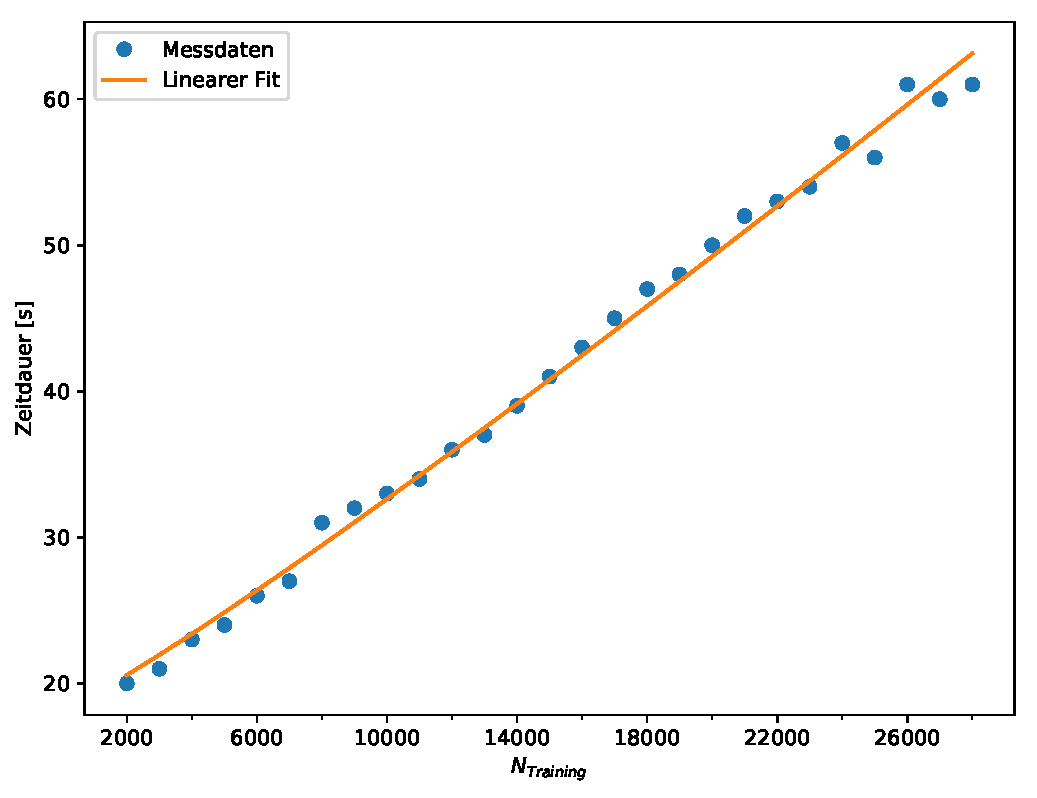
\includegraphics[width=.76\textwidth]{figures/results/cross_prediction/nn_trainlength_uv_time.pdf}
		\caption{Abhängigkeit der Laufzeit von $N_{Training}$.}
	\end{subfigure}%
	\\
	\begin{subfigure}{.95\textwidth}
		\centering
		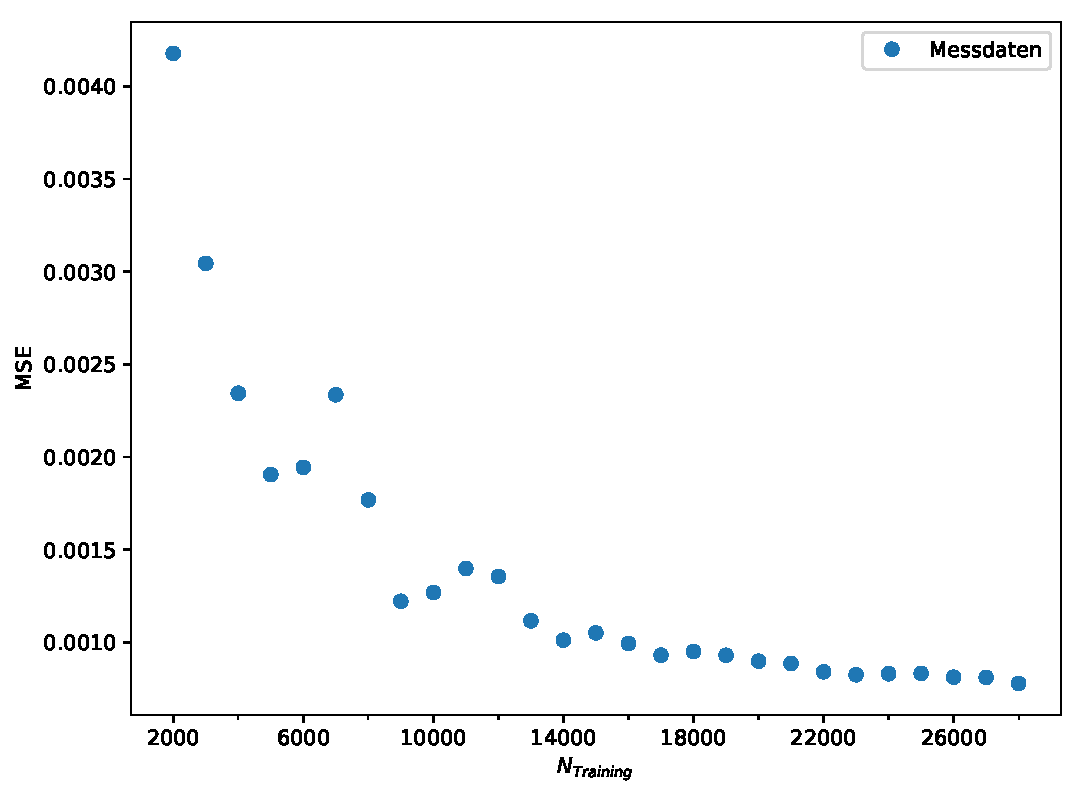
\includegraphics[width=.80\textwidth]{figures/results/cross_prediction/nn_trainlength_uv_mse.pdf}
		\caption{Abhängigkeit des \textit{MSE}s von $N_{Training}$.}
	\end{subfigure}%
	\caption{Darstellung der Abhängigkeit der benötigten Laufzeit (oben) und des MSE (unten) von der verwendeten Anzahl an Trainingsdaten $N_{Training}$ für das \textit{Barkley}-Modell bei der Benutzung einer \textit{Nächsten-Nachbar}-Vorhersage.}
	\label{fig:exp_cross_nn_trainlength_mse_time_barkley}
\end{figure}


\FloatBarrier
\subsection{Radiale Basisfunktionen}
Bei der Verwendung \textit{radialer Basisfunktionen} stellt zudem sowohl die Breite $\sigma_{RBF}$ der Gaußfunktionen als auch die Anzahl der Basisfunktionen $l$ einen wichtigen Parameter dar. Im Rahmen dieser Arbeit ist die Anzahl der Basisfunktionen auf $l=100$ festgelegt worden - diese Wahl wird im Folgenden weiter motiviert werden. Um die anderen Parameter zu finden, sind $\sigma$ und $\Delta \sigma$ wie oben beschrieben, $\delta \in \{3,4,5\}$ und $\sigma_{RBF} \in \{0.5, 1.0, 3.0, 5.0, 7.0, 9.0\}$ variiert worden. In Tabelle \ref{tab:exp_cross_rbf_results} sind die dadurch gefundenen optimalen Parameter, die damit erreichten Fehler und die benötigte Laufzeit erneut für beide Modelle aufgelistet. Wichtig zu sagen ist, dass die optimalen Werte für $\sigma$, $\Delta \sigma$ und $\delta$ mit denen für die NN-Vorhersage übereinstimmen. 

\begin{table}[h]
	\centering

	\begin{tabular}{ccc}
		\hline 			
		\multicolumn{1}{c}{} & Barkley & Mitchell-Schaeffer \\ 
		\hline 
		\rule[-1ex]{0pt}{2.5ex} $\sigma$ & $1$ & $7$ \\ 
		\rule[-1ex]{0pt}{2.5ex} $\Delta \sigma$ & $1$ & $1$ \\ 
		\rule[-1ex]{0pt}{2.5ex} $\delta$ & $3$ & $3$ \\ 
		\rule[-1ex]{0pt}{2.5ex} $\sigma_{RBF}$ & $0.5$ & $5$ \\ 
		\rule[-1ex]{0pt}{2.5ex} Laufzeit [s] & $1430$ & $1434$ \\ 
		\rule[-1ex]{0pt}{2.5ex} \textbf{MSE} & \textbf{0.01046} & \textbf{0.00948} \\ 
		\rule[-1ex]{0pt}{2.5ex} \textbf{NRMSE} & \textbf{0.1023} & \textbf{0.6228} \\ 
		\hline 
	\end{tabular} 
	\caption{Ermittelte Hyperparameter der radialen Basisfunktionen für das \textit{Mitchell-Schaeffer}- und das \textit{Barkley}-Modell, welche zu den geringsten Fehlern führen.}
	\label{tab:exp_cross_rbf_results}
\end{table} 

Analog zu der Untersuchung des Einflusses der Trainingslänge $N_{Training}$ bietet es sich für die radialen Basisfunktionen an, den Einfluss der Anzahl der verwendeten Basisfunktionen $l$ auf die Genauigkeit und die benötigte Laufzeit zu untersuchen, um die zuvor angegebene Wahl $l=100$ zu begründen. Dabei werden die besten zuvor ermittelten Hyperparameter verwendet. Hierfür sind die gemessenen Laufzeiten gegen die Anzahl der Basisfunktionen $l$ in Abbildung \ref{fig:exp_cross_rbf_placements_time_barkley} für das \textit{Barkley}-Modell aufgetragen worden. Zusätzlich ist auch der Zusammenhang zwischen dem erreichten MSE und der Anzahl der Basisfunktionen in Abbildung \ref{fig:exp_cross_rbf_placements_mse_barkley} aufgetragen. Eine dazu analoge Darstellung für das \textit{Mitchell-Schaeffer}-Modell ist in Abbildung \ref{fig:apx_exp_cross_rbf_placements_time_mse_ms} zu finden. Es ist anzunehmen, dass näherungsweise ein linearer Zusammenhang zwischen der Laufzeit und der Anzahl der Basisfunktionen auf dem untersuchten Bereich besteht.\\

\begin{figure}[H]
	\centering
	\begin{subfigure}{\textwidth}
		\centering
		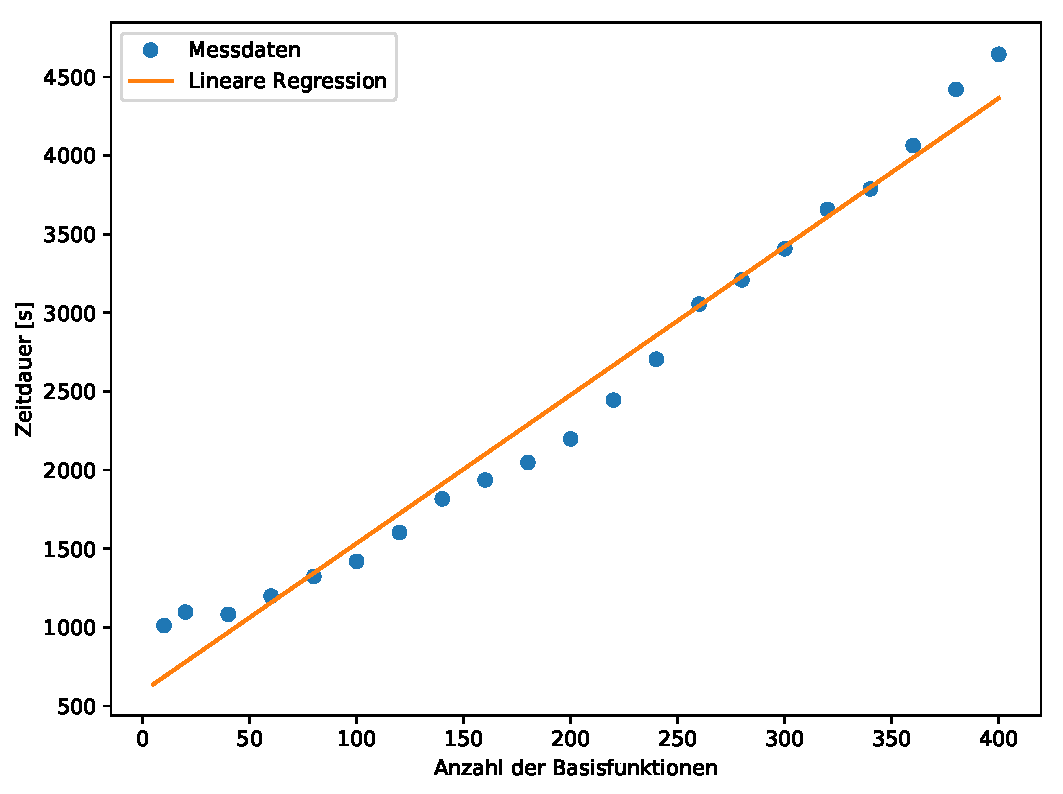
\includegraphics[width=4.2in]{figures/results/cross_prediction/rbf_placements_uv_time.pdf}
		\caption{Abhängigkeit der Laufzeit von $l$.}
		\label{fig:exp_cross_rbf_placements_time_barkley}
	\end{subfigure}%
	\\
	\begin{subfigure}{\textwidth}
		\centering
		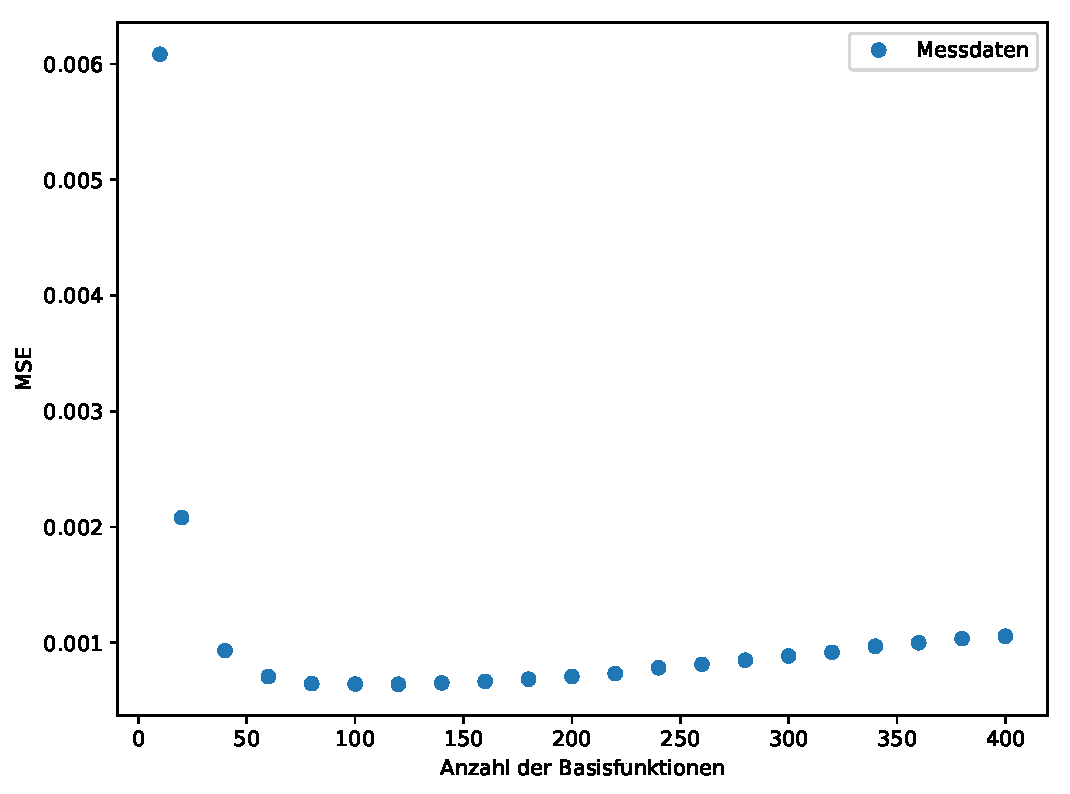
\includegraphics[width=4.2in]{figures/results/cross_prediction/rbf_placements_uv_mse.pdf}
		\caption{Abhängigkeit des Fehlerwertes \textit{MSE} von $l$.}
		\label{fig:exp_cross_rbf_placements_mse_barkley}
	\end{subfigure}%
	\caption{Darstellung der Abhängigkeit der benötigten Laufzeit (oben) und des Fehlerwertes \textit{MSE} von der Anzahl der Basisfunktionen $l$ für das \textit{Barkley}-Modell bei der Verwendung radialer Basisfunktionen.}
\end{figure}

Bei der Untersuchung des Zusammenhangs zwischen MSE und der Anzahl der Basisfunktionen ist zum einen ein asymptotischer Anteil zu sehen, sodass der Fehler zuerst für mehr Basisfunktionen abnimmt. Zum anderen lässt das Verhalten für das \textit{Barkley}-Modell erahnen, dass es hierbei einen optimalen Wert gibt, ab dem der Fehler wieder ansteigt. Dies kann durch eine schlechtere Generalisierung der Dynamik und ein zu starkes Anpassen an die Trainingsdaten (auch bekannt als \textit{Overfitting}) erklärt werden. Daraus resultiert, dass die Wahl von $100$ Basisfunktionen eine akzeptable Abschätzung ist, sodass sowohl der Fehler als auch die Laufzeit möglichst gering gehalten wird. Diese Annahme wird im Folgenden ohne weitere qualitative Untersuchungen auf die anderen beiden Probleme übertragen, um den benötigten Rechenaufwand für die Parametersuche in einem angebrachten Rahmen zu halten.  

\FloatBarrier
\clearpage
\subsection{Echo State Network}
Abschließend ist dieses Problem nun mit den \textit{ESN}s gelöst worden. Dazu sind die Hyperparameter nach Abschnitt \ref{sec:exp_general_esn} gesucht worden. Die gefundenen Parameter und die damit erreichten Ergebnisse sind in Tabelle \ref{tab:exp_cross_esn_results} aufgelistet. Es ist auffällig, dass die optimalen Werte für $\sigma$ und $\Delta \sigma$ hier von denen der NN- und der RBF-Vorhersage abweichen. Des Weiteren ist es erstaunlich, dass für beide Modelle die gleichen Hyperparameter die höchste Genauigkeit erzielen.\improvement{Add more details?} \\

\begin{table}[h]
	\centering
	\captionsetup{width=0.9\linewidth}
	\begin{tabular}{ccc}
		\hline		
		\multicolumn{1}{c}{} &  Barkley & Mitchell-Schaeffer \\ 
		\hline 
		\rule[-1ex]{0pt}{2.5ex} $\sigma$ & $3$ & $3$ \\ 
		\rule[-1ex]{0pt}{2.5ex} $\Delta \sigma$ & $1$ & $1$ \\ 
		\rule[-1ex]{0pt}{3.5ex} $N$ & $400$ & $400$ \\ 
		\rule[-1ex]{0pt}{3.5ex} $\rho(|\mathbf{W}|)$ & $0.95$ & $0.95$\\ 
		\rule[-1ex]{0pt}{3.5ex} $\alpha$ & $0.05$ & $0.05$ \\ 
		\rule[-1ex]{0pt}{3.5ex} $\epsilon$ & $0.1$ & $0.1$ \\ 
		\rule[-1ex]{0pt}{3.5ex} $\nu_{max}$ & $\num{1e-4}$ & $\num{1e-4}$\\ 
		\rule[-1ex]{0pt}{3.5ex} $\lambda$ & $\num{5e-6}$ & $\num{5e-6}$\\ 
		\rule[-1ex]{0pt}{2.5ex} Laufzeit [s] & $3710$ & $3733$ \\ 
		\rule[-1ex]{0pt}{2.5ex} \textbf{MSE} & \textbf{$\num{8.7e-7}$} & \textbf{0.00075} \\ 
		\rule[-1ex]{0pt}{2.5ex} \textbf{NRMSE} & \textbf{0.0039} & \textbf{0.1859} \\ 
		\hline 
	\end{tabular} 
	\caption{Ermittelte Hyperparameter des \textsc{ESN} für das \textit{Mitchell-Schaeffer}- und das \textit{Barkley}-Modell, welche zu den geringsten Fehlern führen.}
	\label{tab:exp_cross_esn_results}
\end{table}

Zusätzlich wird in diesem Szenario auch noch das kompliziertere \textit{BOCF}-Modell betrachtet. Die Vorhersagen in diesem Modell stellen eine größere Herausforderung dar, da es nicht nur über zwei sondern vier Systemvariablen verfügt.\\
Im Folgenden soll nun die Kreuzvorhersage von der $u(t)$ Variable ausgehend auf die $v(t)$, $w(t)$ und $s(t)$ Variable durchgeführt werden. Dazu sind analog zu den anderen beiden Modellen die Hyperparameter nach Abschnitt \ref{sec:exp_general_esn} gesucht worden. Ein graphischer Vergleich zwischen den echten Variablen und den getroffenen Vorhersagen ist in Abbildung \ref{fig:exp_cross_bocf_results} zu finden. Die gefundenen Parameter und die damit erreichten Ergebnisse sind in Tabelle \ref{tab:exp_cross_bocf_results} aufgelistet. \\

\begin{figure}[H]
	\begin{subfigure}{0.5\textwidth}
		\centering
		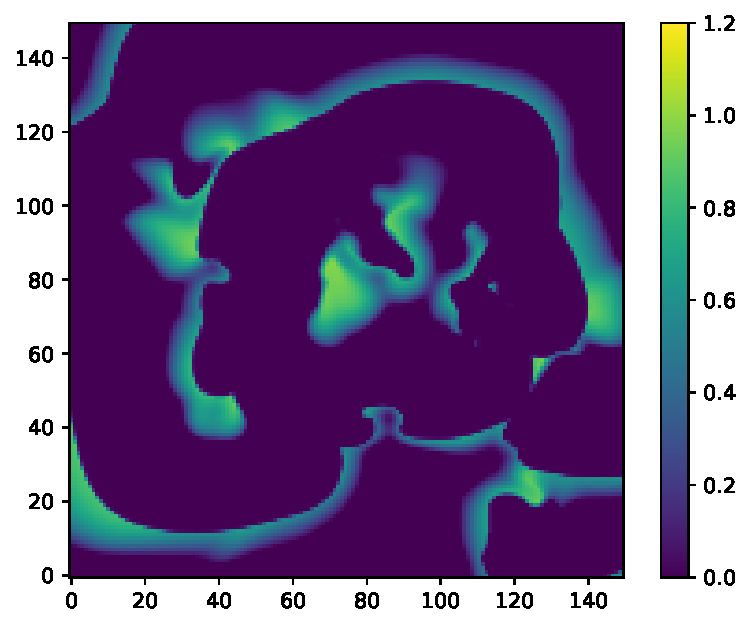
\includegraphics[height=2.5in]{figures/results/cross_prediction/bocf_uv_orig.pdf}
		\caption{Echte Variable $v$}
	\end{subfigure}%
	\begin{subfigure}{0.5\textwidth}
		\centering
		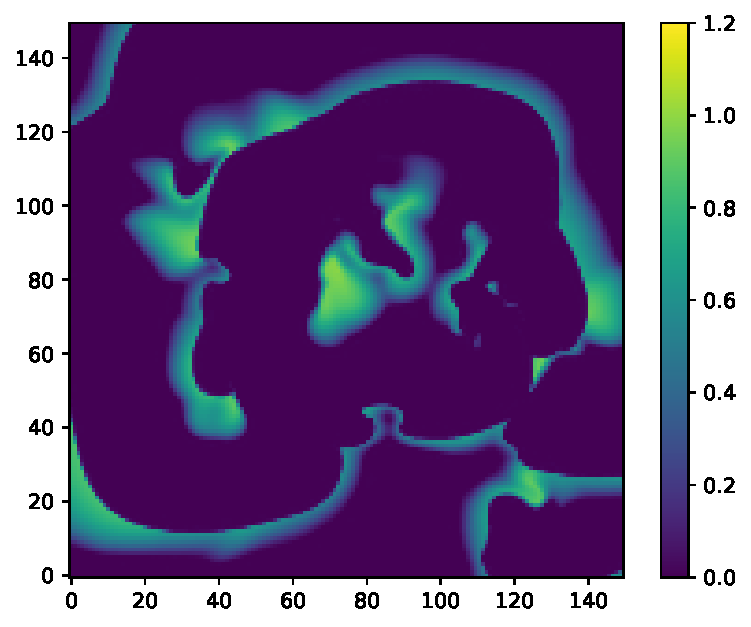
\includegraphics[height=2.5in]{figures/results/cross_prediction/bocf_uv_pred.pdf}
		\caption{Vorhergesagte Variable $v$}
	\end{subfigure}%
	\\
	\begin{subfigure}{0.5\textwidth}
		\centering
		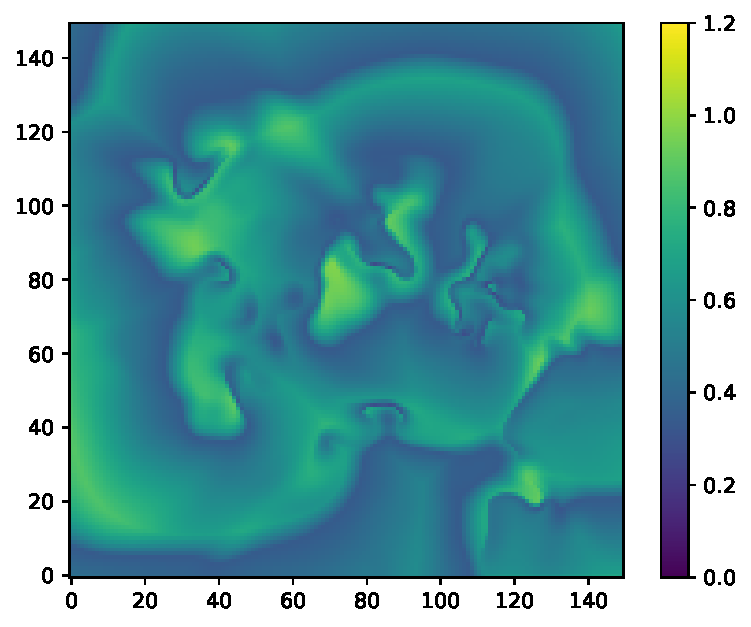
\includegraphics[height=2.5in]{figures/results/cross_prediction/bocf_uw_orig.pdf}
		\caption{Echte Variable $w$}
	\end{subfigure}%
	\begin{subfigure}{0.5\textwidth}
		\centering
		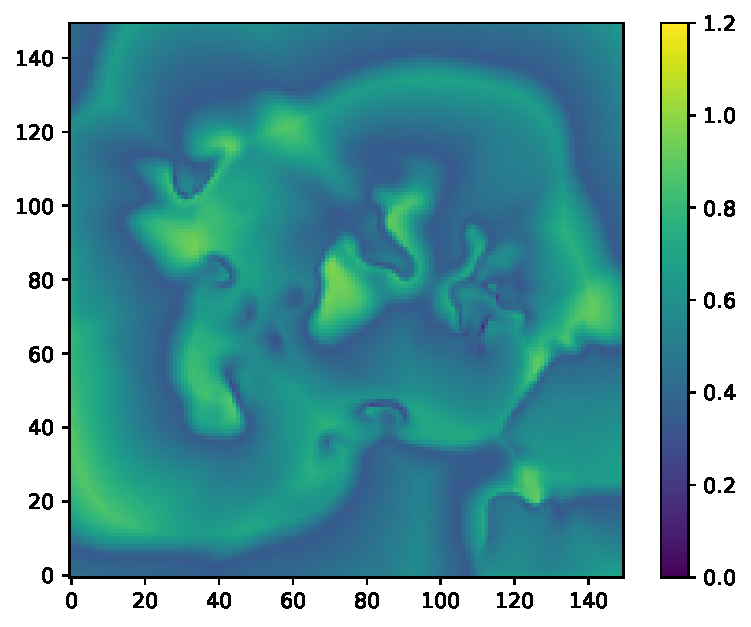
\includegraphics[height=2.5in]{figures/results/cross_prediction/bocf_uw_pred.pdf}
		\caption{Vorhergesagte Variable $w$}
	\end{subfigure}%
	\\
	\begin{subfigure}{0.5\textwidth}
		\centering
		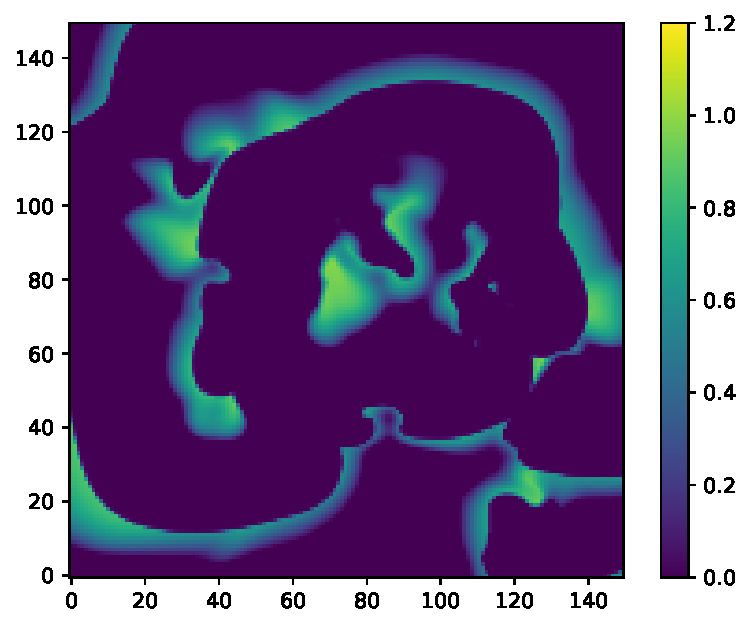
\includegraphics[height=2.5in]{figures/results/cross_prediction/bocf_us_orig.pdf}
		\caption{Echte Variable $s$}
	\end{subfigure}%
	\begin{subfigure}{0.5\textwidth}
		\centering
		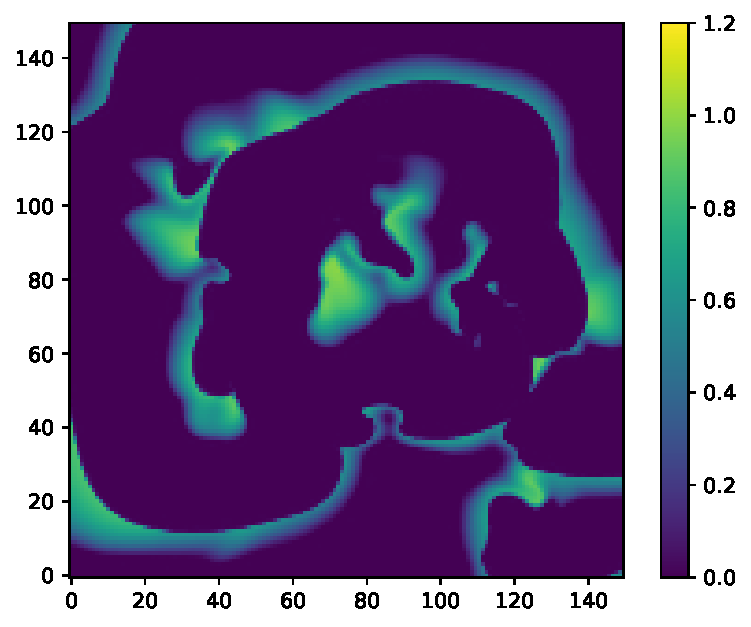
\includegraphics[height=2.5in]{figures/results/cross_prediction/bocf_us_pred.pdf}
		\caption{Vorhergesagte Variable $s$}
	\end{subfigure}%
	\caption{Darstellung der drei verschiedenen Variablen $v(n), w(n), s(n)$ des \textit{BOCF}-Modells bei der Kreuzvorhersage mittels \textsc{ESN} für den Zeitpunkt $n=1000$ des Testdatensatzes. In der linken Spalte ist jeweils die echte Variable und in der rechten die Vorhersage dargestellt.}
	\label{fig:exp_cross_bocf_results}
\end{figure}

\begin{table}[H]
	\centering
	\captionsetup{width=0.9\linewidth}
	\begin{tabular}{cccc}
		\hline		
		\multicolumn{1}{c}{} &  $u(t) \rightarrow v(t)$ & $u(t) \rightarrow w(t)$ & $u(t) \rightarrow s(t)$\\ 
		\hline 
		\rule[-1ex]{0pt}{2.5ex} $\sigma$ & $1$ & $3$ & $1$\\ 
		\rule[-1ex]{0pt}{2.5ex} $\Delta \sigma$ & $1$ & $1$ & $1$ \\ 
		\rule[-1ex]{0pt}{3.5ex} $N$ & $50$ & $400$ & $50$ \\ 
		\rule[-1ex]{0pt}{3.5ex} $\rho(|\mathbf{W}|)$ & $1.10$ & $0.95$ & $1.10$\\ 
		\rule[-1ex]{0pt}{3.5ex} $\alpha$ & $0.95$ & $0.05$ & $0.95$ \\ 
		\rule[-1ex]{0pt}{3.5ex} $\epsilon$ & $0.1$ & $0.1$ & $0.1$ \\ 
		\rule[-1ex]{0pt}{3.5ex} $\nu_{max}$ & $\num{1e-5}$ & $\num{1e-4}$ & $\num{1e-5}$\\ 
		\rule[-1ex]{0pt}{3.5ex} $\lambda$ & $\num{5e-6}$ & $\num{5e-3}$ & $\num{5e-6}$\\ 
		\rule[-1ex]{0pt}{2.5ex} Laufzeit [s] & $1598$ & $3785$ & $1576$ \\ 
		\rule[-1ex]{0pt}{2.5ex} \textbf{MSE} & \textbf{$\num{0.00041}$} & \textbf{0.00009} & $0.00041$ \\ 
		\rule[-1ex]{0pt}{2.5ex} \textbf{NRMSE} & \textbf{0.0716} & \textbf{0.0616} & \textbf{0.0716} \\ 
		\hline 
	\end{tabular} 
	\caption{Ermittelte Hyperparameter des \textsc{ESN} für das \textit{BOCF}-Modell, welche zu den geringsten Fehlern führen.}
	\label{tab:exp_cross_bocf_results}
\end{table}

Es ist zu erkennen, dass eine Kreuzvorhersage mit einen \textsc{ESN} möglich ist und zu einem akzeptablem Fehler führt, welcher in einem ähnlichen Bereich liegt wie bei den Modellen mit zwei Systemvariablen. Deswegen ist anzunehmen, dass auch bei den folgenden zwei Szenarien eine ähnliche Vorhersagequalität, wie bei den anderen beiden Modellen, erreicht werden kann. Für die Vorhersage der $v(t)$ und der $s(t)$ Variable führen identische Hyperparameter zu den genausten Vorhersagen. Auf Grund dieser Beobachtung ist es auch denkbar, dass für ein zugrunde liegendes System mit mehr als zwei Variablen eine Wahl von Hyperparametern existiert, die für beliebige Richtungen der Kreuzvorhersage gute Ergebnisse liefert. Um den Rahmen der Arbeit nicht zu übersteigen, muss auf die Untersuchung dieser Fragestellung verzichtet werden; allerdings wird empfohlen sie in einer weiterführende Arbeit zu untersuchen.\\ 


Zuvor ist die Annahme getroffen worden, dass die Dynamik sich an jedem Punkt im Inneren des Feldes lokal ähnelt. Um diese Annahme zu untersuchen, bietet es sich an, die unterschiedlichen trainierten Gewichtsmatrizen $\mathbf{W_{out}}$ zu betrachten. Dies ist exemplarisch für die ermittelten Hyperparameter für das \textit{Barkley}-Modell durchgeführt und in Abbildung \ref{fig:exp_cross_esn_weights} dargestellt. Dabei gibt die vertikale Achse den Index $i$ des $i$-ten Eintrages von $\mathbf{W_{out}}$ an. Dafür sind die Matrizen $\mathbf{W_{out}} \in \mathbb{R}^{(1 + N_u + N) \times 1}$ mit $N_u = 9$ jeweils spaltenweise für $900$ Pixel in einem $30 \times 30$ Einheiten messendem Quadrat in der Mitte des Feldes aufgetragen.
\improvement{Write something about the vanishing first 9 entries?}

\begin{figure}[H]
	\centering
	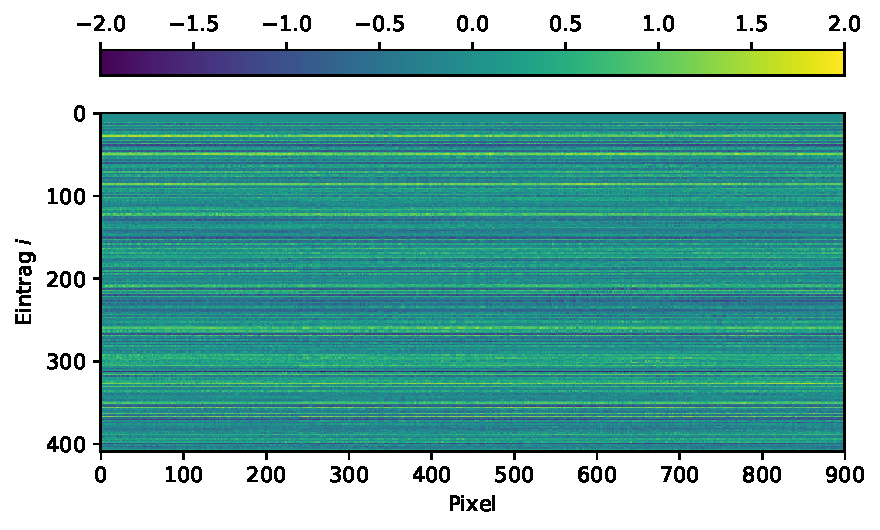
\includegraphics[height=3.0in]{figures/results/cross_prediction/weights.pdf}
	\setcapmargin[1cm]{1cm}
	\caption{Exemplarische Darstellung der Einträge der Gewichtsmatrix $\mathbf{W_{out}}$ des \textsc{ESN} für das \textit{Barkey}-Model anhand von $900$ verschiedene Bildpunkten, wobei $\mathbf{W_{out}}$ jeweils als Spalte in der Grafik dargestellt ist.}
	\label{fig:exp_cross_esn_weights}
\end{figure}



Dabei ist eine große Ähnlichkeit innerhalb der einzelnen Matrizen zu erkennen. Es sind einige markante horizontale Linien in der Abbildung ersichtlich. So sind gewisse Einträge bei den Matrizen aller Pixel relativ stark beziehungsweise schwach. Trotzdem ist noch eine leichte Varianz zuerkennen. Vermutlich wird sie dadurch verursacht, dass innerhalb der endlichen Trainingszeit nicht alle Dynamiken an jedem Pixel auftreten. Zusammenfassend kann dies als eine Bestätigung der Annahme der lokalen Ähnlichkeit gesehen werden. In weiteren Arbeiten bietet es sich an, auch diese Frage weiter zu untersuchen und den Effekt dahingehend auszunutzen, sodass die Trainingsdaten mehrerer Punkte zusammengefasst werden können, damit bereits aus einer kurzen Trainingszeit eine ausreichende Menge an Trainingsdaten gewonnen werden kann. Zudem ist es denkbar, nur noch für einen einzelnen Punkt den Trainingsvorgang durchzuführen, und die folglich bestimmte Gewichtsmatrix $\mathbf{W_{out}}$ für alle Bildpunkte zu nutzen. Dies führt zu einer Reduktion der Gesamtlaufzeit.

\FloatBarrier
\subsection{Vergleich}
Abschließend ist es möglich die drei verwendeten Methoden hinsichtlich ihrer Laufzeit und der erzielten Genauigkeiten zu vergleichen. Dieser ist in Tabelle \ref{tab:exp_cross_comparison_results} zu finden. Die jeweils  besten Ergebnisse sind hervorgehoben. Die \textit{ESN}s erzielen für beide Modelle den geringsten Fehler, also die höchste Genauigkeit. Dabei ist der NRMSE für das \textit{Barkley}-Modell mehrere Größenordnung kleiner als bei den Konkurrenz-Ansätzen. Für das \textit{Mitchell-Schaeffer}-Modell ist diese überaus hohe Genauigkeit nicht erreicht worden. Hier beträgt der Fehler trotzdem etwa nur ein Drittel von dem der anderen Ansätze. Im Austausch für die hohe Genauigkeit ist allerdings die benötigte Zeit für die Vorhersage höher als bei den Konkurrenten. Unter der Voraussetzung, dass die Gesamtlaufzeit nur eine untergeordnete Rolle spielt, erweisen sich die \textit{ESN}s als bester Ansatz für die Kreuzvorhersage.
\begin{table}[h]
	\centering
	\captionsetup{width=0.9\linewidth}
	\begin{tabular}{cccccccc}
		\hline		
		\multicolumn{1}{c}{} & \multicolumn{3}{c}{Barkley} & \multicolumn{3}{c}{Mitchell-Schaeffer}		\\
		%\cline{2-7}
		\multicolumn{1}{c}{} & NN & RBF & ESN & NN & RBF & ESN \\
		
		\hline
		
		Laufzeit [s] 	& \textbf{40} 		& 1430		& 3710		& 5252		& \textbf{1434} 		& 3733 \\
		MSE 			& 0.00098	& 0.01046	& \textbf{\num{8.7e-7}} 	& 0.01891	& 0.00948 	& \textbf{0.00075} \\
		NRMSE 			& 0.1317	& 0.1023	& \textbf{\num{0.0039}} 	& 0.8795	& 0.6228 	& \textbf{0.1859} \\
		\hline 
	\end{tabular} 
	\caption{Vergleich der benötigten Laufzeit und des erreichten Fehlers der drei Ansätze für das \textit{Mitchell-Schaeffer}- und das \textit{Barkley}-Modell, welche zu den geringsten Fehlern führen.}
	\label{tab:exp_cross_comparison_results}
\end{table}

\FloatBarrier